
\chapter{Measuring compiler framework performance}
\label{chap:measuring-compiler-performance}


% Intro

% End-to-end/pipeline-phase-wise performance of xDSL as it stands
% --> Why we pick pattern rewriting to focus on
\section{Compiler pipeline phases}

\section{Micro-benchmarks}
\label{sec:ubenchmark}

% Hook
Micro-benchmarking refers measuring the performance of fast, granular, and isolated segments of code.
% It contrasts traditional benchmarking approaches which instead examine the performance of larger code segments, typically representative of a real-world workload.
% Argument
The term was coined by Saavedra et al. in their 1995 paper \cite{saavedraPerformanceCharacterizationOptimizing1995} ``Performance Characterization of Optimizing Compilers''. As such, we are in good company in our application of micro-benchmarking approaches to this problem domain.
Micro-benchmarks have many desirable properties. Since they run quickly, they can cheaply be repeated for statistical confidence.
Furthermore, their fine granularity makes them tractable to reason about -- providing useful information to optimise the component of the system they measure.
However, a key difficulty of micro-benchmarking is ensuring alignment with overall system performance. For example, the selection of code paths to micro-benchmark may introduce bias, making them less representative of the overall system. In addition to this, their performance may be inflated as a consequence of warmed caches and JIT optimisations across repeats, which would not occur during normal operation.
% Link
As such, micro-benchmarking is a useful tool for deeply understanding the performance of software, but must be used carefully to ensure the validity of its results.

%% Now the mlir community already disagree (cannot find source for this feeling, so elide), leading to talk
% Hook
At the 2024 European LLVM Developers' Meeting, Mehdi Amini and Jeff Nui
presented their keynote talk ``How Slow is MLIR?'' \cite{aminiHowSlowMLIR2024}.
% Argument
In this talk, they discussed micro-benchmarks for key operations in the MLIR compiler, such as traversing the IR and creating operations. These micro-benchmarks were used to inform the optimisation of MLIR's data structures and for comparison with traditional LLVM-based compilers. The implementation of the micro-benchmarks allude to an underlying design goal in MLIR by their measurement of asymptotic scaling properties\footnote{\url{https://github.com/joker-eph/llvm-project/blob/6773f827b9ee8055063fcf6b2c6fcdc7f4f579d2/mlir/unittests/Benchmarks/Cloning.cpp\#L66}}. This design goal is asymptotically optimal performance for its underlying data structures. However, data structures with these characteristics often incur constant-time penalties. % TODO: \cite{}
This causes overhead for small workloads, where, unlike the asymptotic case, the cost is not amortised. As such, micro-benchmarks may not be representative of the system's overall performance, revealing possibility for the optimisation of code co-designed using them.
Despite this, they can still provide useful insight into MLIR's performance characteristics. 
% Link
We implement micro-benchmark workloads for the xDSL equivalent to those for MLIR presented in the keynote, and compare the results of these benchmarks between the two implementations, giving insights into their relative performance.
% We further leverage profiling tools to examine the execution of the two implementations. This allows us to distinguish the cost incurred by the language runtime from the cost incurred by the algorithmic approach of the implementation.


\subsection{Methodology}
\label{ssec:ubenchmark-methodology}

% Hook
Our experimental methodology aims to maximize the effectiveness of micro-benchmarks while minimising their inherent limitations.
% Argument
To achieve this balance, we developed infrastructure for benchmark execution and carefully implemented measurement logic.
This approach ensures that our measurements accurately reflect overall system performance and ensure valid comparisons between implementations.
% Link

\subsubsection{Micro-benchmarking infrastructure}
\label{sssec:ubenchmark-methodology-infra}

% Hook
Due to their short length, micro-benchmark results are sensitive to machine noise.
% Argument
To minimise the impact of machine noise, the micro-benchmarks are repeated $2^{15}$ times and averaged, with uncertainty calculated as their standard deviation. To ensure comparability, both the MLIR and xDSL micro-benchmarks were run locally on the same experimental machine, whose hardware and software configuration is described in \autoref{tab:ubenchmark-experimental-config}
% % Link
% In addition to machine noise, other mechanisms may increase the variance of results, such as differences between runs due to cache warming or language runtime behaviour.

\begin{table}[H]
  \caption{Experimental configuration used for micro-benchmarking.}
  % TODO: This might want to move to the top of the measurement section?
  \label{tab:ubenchmark-experimental-config}
  \centering
  \begin{tabular}{lll}
    \toprule
    \textbf{Configurable} & \textbf{Configuration} \\
    \midrule
    \textit{xDSL commit SHA} & \texttt{0eda7fe} \\
    \textit{MLIR commit SHA} & \texttt{6516ae4} \\
    \midrule
    % \midrule  % Build/run command here???
    % `python3 benchmarks/microbenchmarks.py Extensibility.trait_check`
    % `cmake ...`
    % `./MLIR_IR_Benchmark --benchmark_filter="NAME/32768" --benchmark_repetitions=10
    \textit{Python interpreter} & CPython 3.12.9 \\
    \textit{C++ compiler} & clang 18.1.8 \\
    \textit{CMake version} & 3.31.3 \\
    \textit{Ninja version} & 1.12.1 \\
    \textit{Operating system} & macOS Sequoia 15.4.1 \\
    \midrule
    % \textit{Clock frequency [GHz]} & \\
    \textit{CPU} & Apple M3 \\
    \textit{RAM [GB]} & 16 \\
    \bottomrule
  \end{tabular}
\end{table}

%% TODO: This might move to end-to-end benchmarks section?
% Hook
In addition to their usefulness for understanding and optimising compiler performance, these benchmarks provide an opportunity to augment the development process of the xDSL project.
% Argument
Benchmarks can be used to characterise the performance impact of changes to the xDSL codebase, making it easier to avoid unnecessary performance regression.
As such, we provide a command line interface for developers to run the benchmarks, with further functionality which supports a variety of profiling tools.
Furthermore, our benchmarks are constructed to interface with air-speed velocity \cite{michaeldroettboomAirspeedvelocityAsv2025}, a tool which runs benchmarks across repository commits. This information is tracked on the xDSL website \url{https://xdsl.dev/xdsl-bench/}, providing a dashboard for the performance characteristics of xDSL over time.
% Link

% Hook
After constructing reliable infrastructure for executing micro-benchmarks in Python, we proceeded to develop implementations that could be directly compared with existing MLIR versions. This was essential to draw valid conclusions about performance differences between Python and C++ runtimes for compiler framework workloads.


\subsubsection{Micro-benchmarking implementation}
\label{sssec:ubenchmark-methodology-impl}

%% Finding and building the MLIR microbenchmarks
% Hook
Unfortunately, the implementation and build instructions for the ``How Slow is MLIR?'' micro-benchmarks were not published with the talk.
% Argument (too informal?)
However, their source code can be found on a branch of the presenter's fork of LLVM\footnote{\url{https://github.com/joker-eph/llvm-project/tree/benchmarks}}. We provide a copy of this source code and instructions for running the benchmarks\footnote{\url{https://github.com/EdmundGoodman/llvm-project-benchmarks}} to enhance the replicability of our results and facilitate further performance experiments.
% Link
This source code can then be used to construct comparable micro-benchmarks in Python.

% Design of our microbenchmarks
% Hook
A key design goal of our micro-benchmarks for xDSL is parity with those provided for MLIR, ensuring the validity their direct comparison.
% Argument
As such, their implementation was derived from the MLIR benchmarks, matching test data and function invocations as closely as possible.
% Link
In the following sections, we discuss the implementations of a number of micro-benchmarks, facilitating discussion of the insights they give into compiler performance across implementations and language runtimes in later chapters.




\subsection{Operation trait checks}
\label{ssec:ubenchmark-trait-checks}

% Hook
MLIR and xDSL both provide methods to check whether operations have traits.
% Argument
These methods are used very frequently in common tasks. For example, when pattern rewriting over a block of IR, the traits of the block's constituent operations are often used by the matching engine to identify valid rewrites.

% There are two factors which contribute to this slow-down. The first is the inherent overhead incurred by the interpreter loop and data structures in Python's dynamic language runtime. The second is differences in implementation between xDSL and MLIR.
% % Link
% Examining this micro-benchmark in detail allows us to decouple the performance contributions of the implementation and language runtime, and provides insight into the impact of dynamism on user-extensible compiler framework workloads.

\begin{figure}[H]
    \centering
    \begin{subfigure}[b]{0.45\textwidth}
       \centering
        \begin{minted}[fontsize=\footnotesize]{c++}
            // Setup
            Operation op = b.create<OpWithRegion>(
                unknownLoc
            );
            
            // Benchmark
            bool hasTrait = op->hasTrait<
                OpTrait::SingleBlock
            >();
        \end{minted}
        \caption{``How Slow is MLIR?'' C++ implementation.}
        \label{listing:ubenchmark-trait-checks-bench-mlir}
    \end{subfigure}
    \hfill
    \begin{subfigure}[b]{0.45\textwidth}
        \centering
        \begin{minted}[breakanywhere,fontsize=\footnotesize]{python}
            # Setup
            op = OpWithRegion()
            
            # Benchmark
            has_trait = op.has_trait(SingleBlock)
        \end{minted}
        \footnotesize\vspace{2em}
        \caption{xDSL Python implementation.}
        \label{listing:ubenchmark-trait-checks-bench-xdsl}
    \end{subfigure}
    \vspace{1em}
    \captionsetup{name=Listing}
    \caption{Micro-benchmark implementations for methods checking an operation has a trait.}
    \label{listing:ubenchmark-trait-checks-bench}
\end{figure}

Micro-benchmarks of checking traits for both implementations (Listing \ref{listing:ubenchmark-trait-checks-bench}) show a slow-down of approximately $130\times$ from MLIR to xDSL (\autoref{tab:ubenchmark-trait-checks}).

\begin{table}[H]
  \caption{Trait checks in xDSL are approximately $130\times$ slower than in MLIR in the asymptotic case.} %, repeated ten times over $32768$ operations. Methodology is discussed in detail in Appendix \ref{} to facilitate replicability.}
  \label{tab:ubenchmark-trait-checks}
  \centering
  \begin{tabular}{cc}
    \toprule
    \textbf{MLIR [ns]} & \textbf{xDSL [ns]}\\
    \midrule
    $3.89 \pm 0.01$ & $504 \pm 76$ \\
    \bottomrule
  \end{tabular}
\end{table}


% % Hook
% The trait checking micro-benchmark yields two key insights.
% % Argument
% The first is that the original implementation of xDSL makes significant tradeoffs of performance for expressivity. By eliminating these tradeoffs, we reveal the Python language runtime incurs a $16\times$ overhead with respect to C++, as a result of the complexity of its evaluation loop.
% The second is that whilst C++ can efficiently represent dynamic functionality, albeit at the cost of implementation complexity, dynamism incurs the cost of obscuring other optimisations that would further widen the performance gap between Python and C++.
% % Link
% However, whilst trait checking is a frequent operation, it alone is not representative of the overall performance of compiler frameworks. As such, further micro-benchmarks and examining representative workloads is required.


\subsection{Operation instantiation}

\subsection{Summary of micro-benchmarks}

% Hook
In addition to the above micro-benchmarks which we examine in detail, we further provide a wider suite of micro-benchmarks discussed in lesser detail for brevity. % The implementations of all xDSL micro-benchmarks are provided in the Appendix (\autoref{}).
% Argument
This suite implements many of the remaining equivalent micro-benchmarks from ``How Slow is MLIR'' (\autoref{tab:ubenchmark-remaining-mlir}).
From these, we can see the trend of a slow-down in the order of $xy\times$ holds 

\begin{table}[H]
  \caption{.}
  \label{tab:ubenchmark-remaining-mlir}
  \centering
  \begin{tabular}{ccc}
    \toprule
    \textbf{Benchmark name} & \textbf{MLIR [ns]} & \textbf{xDSL [ns]}\\
    \midrule
    Trait checks & $3.89 \pm 0.01$ & $504 \pm 76$ \\
    ... & ... & ... \\
    \bottomrule
  \end{tabular}
\end{table}


% Hook
In addition to the remaining ``How Slow is MLIR?'' micro-benchmarks, the suite provides further xDSL-only micro-benchmarks sampled from atomic functions invoked by pattern rewriting workloads (\autoref{tab:ubenchmark-xdsl-regression}).
% Argument
These have two-fold use: triaging functions to optimise by longest runtime following Amdhal's law \cite{amdahlValiditySingleProcessor1967}; and serving as a metric of performance to ensure optimisations don't inadvertently introduce regressions.
% Link

\begin{table}[H]
  \caption{.}
  \label{tab:ubenchmark-xdsl-regression}
  \centering
  \begin{tabular}{ccc}
    \toprule
    \textbf{Benchmark name} & \textbf{xDSL [ns]}\\
    \midrule
    Trait checks & $504 \pm 76$ \\
    ... & ... & ... \\
    \bottomrule
  \end{tabular}
\end{table}



\section{Pattern rewriting}



















\chapter{Profiling Python bytecode} % for fun and profit







\chapter{Specialising and optimising xDSL pattern rewriting}

\section{Micro-benchmarks}

% Hook
% Argument
% Link

\subsection{Operation trait checks}

% Hook
Chapter \ref{chap:measuring-compiler-performance} measured a slow-down of approximately $130\times$ from MLIR to xDSL for trait checking micro-benchmarks (\autoref{tab:ubenchmark-trait-checks}).
% Argument
There are two factors which contribute to this slow-down. The first is the inherent overhead incurred by the interpreter loop and data structures in Python's dynamic language runtime. The second is differences in implementation between xDSL and MLIR.
% Link
Examining this micro-benchmark in detail allows us to decouple the performance contributions of the implementation and language runtime.
% , and provides insight into the impact of dynamism on user-extensible compiler framework workloads.

\begin{figure}[H]
    \begin{subfigure}[b]{0.45\textwidth}
       \centering
        \begin{minted}[fontsize=\footnotesize]{python}
            @classmethod
            def has_trait(
                cls,
                trait: type[OpTrait] | OpTrait,
                *,
                value_if_unregistered: bool = True,
            ) -> bool:
                from xdsl.dialects.builtin import UnregisteredOp
        
                if issubclass(cls, UnregisteredOp):
                    return value_if_unregistered
        
                return cls.get_trait(trait) is not None
        \end{minted}
        \footnotesize\vspace{1.5em}
        \caption{Outer \mintinline{python}{has_trait} method.}
        \label{listing:ubenchmark-trait-checks-xdsl-has}
    \end{subfigure}
    \hfill
    \begin{subfigure}[b]{0.45\textwidth}
        \centering
        \begin{minted}[breakanywhere,fontsize=\footnotesize]{python}
            @classmethod
            def get_trait(
                cls,
                trait: type[OpTraitInvT] | OpTraitInvT
            ) -> OpTraitInvT | None:
                if isinstance(trait, type):
                    for t in cls.traits:
                        if isinstance(t, cast(
                            type[OpTraitInvT], trait
                        )):
                            return t
                else:
                    for t in cls.traits:
                        if t == trait:
                            return cast(OpTraitInvT, t)
                return None
        \end{minted}
        \caption{Inner \mintinline{python}{get_trait} method.}
        \label{listing:ubenchmark-trait-checks-xdsl-get}
    \end{subfigure}
    \vspace{1em}
    \captionsetup{name=Listing}
    \caption{xDSL methods implementing trait check functionality.}
    \label{listing:ubenchmark-trait-checks-xdsl}
\end{figure}

% Hook
In order to distinguish between the slow-down incurred by the language runtime as opposed to each approach's implementation, we leverage tracing profilers to examine the call stacks of the micro-benchmarks.
% Argument
In the xDSL implementation of \mintinline{python}{has_trait} (Listing \ref{listing:ubenchmark-trait-checks-xdsl}), we can see that approximately half of the operation is spent checking if the operation subclasses \mintinline{python}{UnregisteredOp} (\autoref{fig:ubenchmark-hastrait-xdsl-viztracer}).
Furthermore, \mintinline{python}{has_trait}s sub-invocation \mintinline{python}{get_trait} further incurs overhead with \mintinline{python}{isinstance} checks, \mintinline{python}{cast}ing and constructing iterators (\autoref{fig:ubenchmark-gettrait-xdsl-viztracer}).
% Link
This demonstrates that a significant proportion of the slow-down in xDSL's \mintinline{python}{has_trait} method is as a result of implementation details, as opposed to inherent limitations of Python's runtime.

\begin{figure}[H]
    \centering
    \begin{subfigure}[b]{\textwidth}
        \centering
        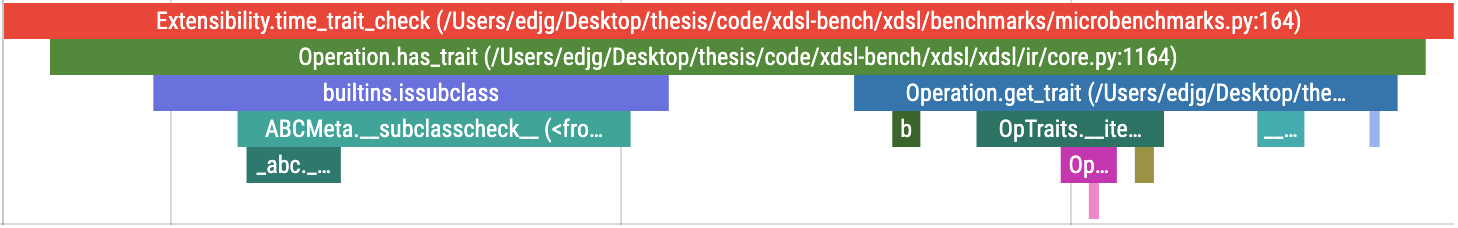
\includegraphics[width=\textwidth]{images/14_understanding_compiler_performance/trait_checks/hastrait_xdsl_viztracer.png}
        \caption{Checking for \mintinline{python}{UnregisteredOp}s constitutes around half of \mintinline{python}{has_trait}s runtime.}
        \label{fig:ubenchmark-hastrait-xdsl-viztracer}
    \end{subfigure}
    \begin{subfigure}[b]{\textwidth}
        \centering
        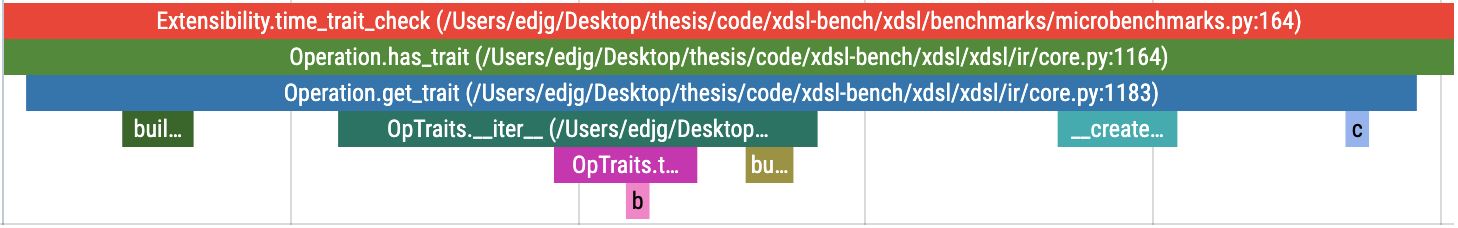
\includegraphics[width=\textwidth]{images/14_understanding_compiler_performance/trait_checks/gettrait_xdsl_viztracer.png}
        \caption{\mintinline{python}{isinstance} checks, \mintinline{python}{cast}ing and constructing iterators constitutes around half of \mintinline{python}{get_trait}s runtime.}
        \label{fig:ubenchmark-gettrait-xdsl-viztracer}
    \end{subfigure}
    \caption{\texttt{viztracer} trace of xDSL's \mintinline{python}{has_trait} and \mintinline{python}{get_trait} methods.}
    \label{fig:ubenchmark-hasgettrait-xdsl-viztracer}
\end{figure}

% Hook
By modifying xDSL's implementation to elide the extraneous code identified in the above traces (Listing \ref{listing:ubenchmark-trait-checks-both-xdsl}), we can improve its performance by a factor of eight (\autoref{tab:ubenchmark-trait-checks-optimised}).
This gives a number of insights into writing performant Python code in cases where it is unsuitable to dispatch to a lower level languages.
% Argument
Firstly, even atomic operations such as function invocation and selection statements are slow in comparison to the runtime of the C++ implementation, coming as a result of the complexity of the evaluation loop of the CPython interpreter. % TODO: Consider \cite{}?
This is substantiated by the bytecode profiles of the implementations (Appendix \ref{listing:bytecode-profiles-hastrait-original}, \ref{listing:bytecode-profiles-hastrait-optimised}), where each opcode represents in iteration of the evaluation loop.
In the case of \mintinline{python}{has_trait}, we address this by manually applying function inlining, and narrowing the trait argument from supporting both types and instances to only supporting types, eliminating selection of implementation between the two arguments. This minimises the number of opcodes and hence the number of cycles of the evaluation loop, improving performance.
% Link
Unfortunately, these approaches are in tension with writing expressive and terse code -- which are motivating factors for using Python.



\begin{table}[H]
  \caption{Trait checks in xDSL are approximately $130\times$ slower than in MLIR in the asymptotic case, but can be accelerated to $16\times$ slower with only algorithmic changes.} %, repeated ten times over $32768$ operations. Methodology is discussed in detail in Appendix \ref{} to facilitate replicability.}
  \label{tab:ubenchmark-trait-checks-optimised}
  \centering
  \begin{tabular}{ccc}
    \toprule
    \textbf{MLIR [ns]} & \textbf{xDSL [ns]} & \textbf{Optimised xDSL [ns]} \\
    \midrule
    $3.89 \pm 0.01$ & $504 \pm 76$ & $63.6 \pm 40$\\
    \bottomrule
  \end{tabular}
\end{table}



\begin{figure}[H]
    \centering
    \begin{subfigure}[b]{0.45\textwidth}
       \centering
        \begin{minted}[fontsize=\footnotesize]{python}
            has_trait = False
            for t in OP.traits._traits:
                if isinstance(t, TRAIT):
                    has_trait = True
                    break
        \end{minted}
        \footnotesize\vspace{5.5em}
        \captionsetup{name=Listing}
        \caption{xDSL's modified \mintinline{python}{has_trait} method.}
        \label{listing:ubenchmark-trait-checks-both-xdsl}
    \end{subfigure}
    \hfill
    \begin{subfigure}[b]{0.45\textwidth}
        \centering
        \begin{minted}[breakanywhere,fontsize=\footnotesize]{c++}
            template <template <typename T> class... Traits>
            inline bool hasTrait(TypeID traitID) {
                TypeID traitIDs[] = {TypeID::get<Traits>()...};
                for (unsigned i = 0, e = sizeof...(Traits); i != e; ++i)
                    if (traitIDs[i] == traitID)
                        return true;
                return false;
            }
            template <>
            inline bool hasTrait<>(TypeID traitID) {
                return false;
            }
        \end{minted}
        \captionsetup{name=Listing}
        \caption{MLIR's \mintinline{c++}{has_trait} method.}
        \label{listing:ubenchmark-trait-checks-both-mlir}
    \end{subfigure}
    \vspace{1em}
    \captionsetup{name=Listing}
    \caption{xDSL and MLIR methods searching trait arrays.}
    \label{listing:ubenchmark-trait-checks-both}
\end{figure}


\subsection{Operation instantiation}



\section{Constant folding workload}












\chapter{Impact of CPython performance enhancements on xDSL pattern rewriting}

\section{Specialising adaptive interpreter}
\section{JIT compilation}
\section{Tail call interpreter}




% \chapter{Ideally final optimisation stuff}





\chapter{Examining the impact of dynamism on pattern rewriting in static and dynamic languages}

\section{Quantifying the performance impact of dynamism on C++}

\section{Dynamism in xDSL}

\subsection{Operation trait checks}

% Hook
Having specialised xDSL's \mintinline{python}{has_trait} method to the most minimal implementation which expresses the desired functionality, we can draw comparisons between equivalent algorithms which predominantly measure the effect of the language runtime.
% Argument
Both implementations (Listing \ref{listing:ubenchmark-trait-checks-both}) share the same underlying algorithm: iteration over an operations traits, checking against each one. However, the mechanism used for this algorithm differs significantly between xDSL and MLIR.
By leveraging Python's dynamic nature, xDSL can invoke the \mintinline{python}{isinstance} function to check each trait. In contrast, MLIR uses template metaprogramming instead of the class hierarchy to define traits. This depends on \mintinline{c++}{TypeID}\footnote{\url{https://mlir.llvm.org/doxygen/TypeID_8h_source.html}}, a custom data structure to encode dynamic \ac{rtti} in C++.
% TODO: Does this need more detail?
Whilst this implementation incurs complexity (\autoref{fig:ubenchmark-hastrait-dynamism}), it remains performant, as the \mintinline{c++}{TypeID} data structure is constructed to remedy many of the issues of native C++ \ac{rtti}.
% Link
However, this dynamism impacts performance beyond just the runtime of the individual function, as it presents an optimisation boundary -- precluding other optimisations which could be applied if the result could be inferred at compile time. % TODO: This really needs to be substantiated somehow, but perhaps not here?

\begin{figure}[H]
    \centering
    \begin{subfigure}[b]{\textwidth}
        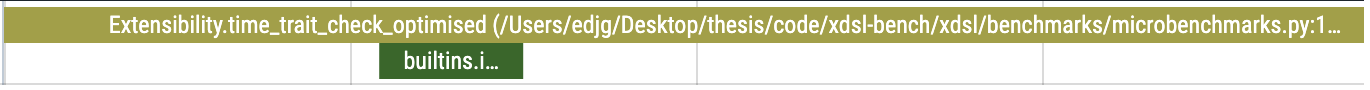
\includegraphics[width=\textwidth]{images/14_understanding_compiler_performance/trait_checks/hastrait_xdsl_viztracer_optimised.png}
        \caption{\texttt{viztracer} trace of xDSL's optimised \mintinline{python}{has_trait} implementation.}
        \label{fig:ubenchmark-hastrait-xdsl-viztracer-optimised}
    \end{subfigure}
    \begin{subfigure}[b]{\textwidth}
        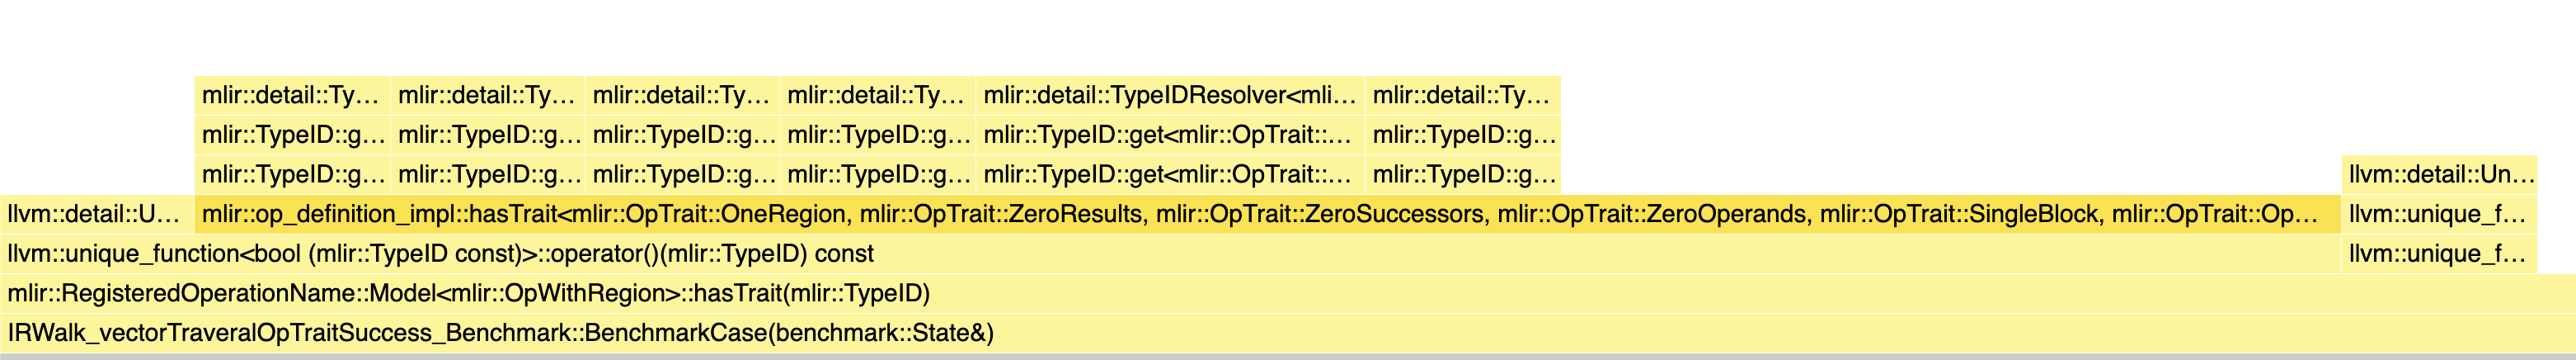
\includegraphics[width=\textwidth]{images/14_understanding_compiler_performance/trait_checks/hastrait_mlir_samply.png}
        \caption{\texttt{samply} trace of MLIR's \mintinline{c++}{has_trait} method.}
        \label{fig:ubenchmark-hastrait-mlir-samply}
    \end{subfigure}
    \caption{MLIR's dynamic trait checking using C++ RTTI is more complex than xDSL's Python implementation using \mintinline{python}{isinstance}.}
    \label{fig:ubenchmark-hastrait-dynamism}
\end{figure}
